%\VignetteIndexEntry{Introduction to the dataRetrieval package}
%\VignetteEngine{knitr::knitr}
%\VignetteDepends{}
%\VignetteSuggests{xtable,EGRET}
%\VignetteImports{zoo, XML, RCurl}
%\VignettePackage{dataRetrieval}

\documentclass[a4paper,11pt]{article}\usepackage[]{graphicx}\usepackage[]{color}
%% maxwidth is the original width if it is less than linewidth
%% otherwise use linewidth (to make sure the graphics do not exceed the margin)
\makeatletter
\def\maxwidth{ %
  \ifdim\Gin@nat@width>\linewidth
    \linewidth
  \else
    \Gin@nat@width
  \fi
}
\makeatother

\definecolor{fgcolor}{rgb}{0.345, 0.345, 0.345}
\newcommand{\hlnum}[1]{\textcolor[rgb]{0.686,0.059,0.569}{#1}}%
\newcommand{\hlstr}[1]{\textcolor[rgb]{0.192,0.494,0.8}{#1}}%
\newcommand{\hlcom}[1]{\textcolor[rgb]{0.678,0.584,0.686}{\textit{#1}}}%
\newcommand{\hlopt}[1]{\textcolor[rgb]{0,0,0}{#1}}%
\newcommand{\hlstd}[1]{\textcolor[rgb]{0.345,0.345,0.345}{#1}}%
\newcommand{\hlkwa}[1]{\textcolor[rgb]{0.161,0.373,0.58}{\textbf{#1}}}%
\newcommand{\hlkwb}[1]{\textcolor[rgb]{0.69,0.353,0.396}{#1}}%
\newcommand{\hlkwc}[1]{\textcolor[rgb]{0.333,0.667,0.333}{#1}}%
\newcommand{\hlkwd}[1]{\textcolor[rgb]{0.737,0.353,0.396}{\textbf{#1}}}%

\usepackage{framed}
\makeatletter
\newenvironment{kframe}{%
 \def\at@end@of@kframe{}%
 \ifinner\ifhmode%
  \def\at@end@of@kframe{\end{minipage}}%
  \begin{minipage}{\columnwidth}%
 \fi\fi%
 \def\FrameCommand##1{\hskip\@totalleftmargin \hskip-\fboxsep
 \colorbox{shadecolor}{##1}\hskip-\fboxsep
     % There is no \\@totalrightmargin, so:
     \hskip-\linewidth \hskip-\@totalleftmargin \hskip\columnwidth}%
 \MakeFramed {\advance\hsize-\width
   \@totalleftmargin\z@ \linewidth\hsize
   \@setminipage}}%
 {\par\unskip\endMakeFramed%
 \at@end@of@kframe}
\makeatother

\definecolor{shadecolor}{rgb}{.97, .97, .97}
\definecolor{messagecolor}{rgb}{0, 0, 0}
\definecolor{warningcolor}{rgb}{1, 0, 1}
\definecolor{errorcolor}{rgb}{1, 0, 0}
\newenvironment{knitrout}{}{} % an empty environment to be redefined in TeX

\usepackage{alltt}

\usepackage{amsmath}
\usepackage{times}
\usepackage{hyperref}
\usepackage[numbers, round]{natbib}
\usepackage[american]{babel}
\usepackage{authblk}
\usepackage{subfig}
\usepackage{placeins}
\usepackage{footnote}
\usepackage{tabularx}
\usepackage{threeparttable}
\usepackage{parskip}

\usepackage{csquotes}
\usepackage{setspace}

\doublespacing

\renewcommand{\topfraction}{0.85}
\renewcommand{\textfraction}{0.1}
\usepackage{graphicx}


\usepackage{mathptmx}% Times Roman font
\usepackage[scaled=.90]{helvet}% Helvetica, served as a model for arial

\usepackage{indentfirst}
\setlength{\parskip}{0pt}

\usepackage{courier}

\usepackage{titlesec}
\usepackage{titletoc}

\titleformat{\section}
  {\normalfont\sffamily\bfseries\LARGE}
  {\thesection}{0.5em}{}
\titleformat{\subsection}
  {\normalfont\sffamily\bfseries\Large}
  {\thesubsection}{0.5em}{}
\titleformat{\subsubsection}
  {\normalfont\sffamily\large}
  {\thesubsubsection}{0.5em}{}
  
\titlecontents{section}
[2em]                 % adjust left margin
{\sffamily}             % font formatting
{\contentslabel{2.3em}} % section label and offset
{\hspace*{-2.3em}}
{\titlerule*[0.25pc]{.}\contentspage}
  
\titlecontents{subsection}
[4.6em]                 % adjust left margin
{\sffamily}             % font formatting
{\contentslabel{2.3em}} % section label and offset
{\hspace*{-2.3em}}
{\titlerule*[0.25pc]{.}\contentspage}
  
\titlecontents{subsubsection}
[6.9em]                 % adjust left margin
{\sffamily}             % font formatting
{\contentslabel{2.3em}} % section label and offset
{\hspace*{-2.3em}}
{\titlerule*[0.25pc]{.}\contentspage}

\titlecontents{table}
[0em]                 % adjust left margin
{\sffamily}             % font formatting
{\textbf{Table}\hspace*{2em} \contentslabel {2em}} % section label and offset
{\hspace*{4em}}
{\titlerule*[0.25pc]{.}\contentspage}

\titlecontents{figure}
[0em]                 % adjust left margin
{\sffamily}             % font formatting
{\textbf{Figure}\hspace*{2em} \contentslabel {2em}} % section label and offset
{\hspace*{4em}}
{\titlerule*[0.25pc]{.}\contentspage}

%Italisize and change font of urls:
\urlstyle{sf}
\renewcommand\UrlFont\itshape

\usepackage{caption}
\captionsetup{
  font={sf},
  labelfont={bf,sf},
  labelsep=period,
  justification=justified,
  singlelinecheck=false
}

\setlength\parindent{20pt}

\textwidth=6.2in
\textheight=8.5in
\parskip=.3cm
\oddsidemargin=.1in
\evensidemargin=.1in
\headheight=-.3in


%------------------------------------------------------------
% newcommand
%------------------------------------------------------------
\newcommand{\scscst}{\scriptscriptstyle}
\newcommand{\scst}{\scriptstyle}
\newcommand{\Robject}[1]{{\texttt{#1}}}
\newcommand{\Rfunction}[1]{{\texttt{#1}}}
\newcommand{\Rclass}[1]{\textit{#1}}
\newcommand{\Rpackage}[1]{\textit{#1}}
\newcommand{\Rexpression}[1]{\texttt{#1}}
\newcommand{\Rmethod}[1]{{\texttt{#1}}}
\newcommand{\Rfunarg}[1]{{\texttt{#1}}}
\IfFileExists{upquote.sty}{\usepackage{upquote}}{}
\begin{document}



\renewenvironment{knitrout}{\begin{singlespace}}{\end{singlespace}}
\renewcommand*\listfigurename{Figures}

\renewcommand*\listtablename{Tables}


%------------------------------------------------------------
\title{The dataRetrieval R package}
%------------------------------------------------------------
\author[1]{Laura De Cicco}
\author[1]{Robert Hirsch}
\affil[1]{United States Geological Survey}




\noindent{\huge\textsf{\textbf{The dataRetrieval R package}}}

\noindent\textsf{By Laura De Cicco and Robert Hirsch}

\noindent\textsf{\today}

% \maketitle
% 
% \newpage 

\tableofcontents
\listoffigures
\listoftables

\newpage

%------------------------------------------------------------
\section{Introduction to dataRetrieval}
%------------------------------------------------------------ 
The dataRetrieval package was created to simplify the process of loading hydrologic data into the R environment. It has been specifically designed to work seamlessly with the EGRET R package: Exploration and Graphics for RivEr Trends. See: \url{https://github.com/USGS-R/EGRET/wiki} for information on EGRET. EGRET is designed to provide analysis of water quality data sets using the Weighted Regressions on Time, Discharge and Season (WRTDS) method as well as analysis of discharge trends using robust time-series smoothing techniques.  Both of these capabilities provide both tabular and graphical analyses of long-term data sets.


The dataRetrieval package is designed to retrieve many of the major data types of United States Geological Survey (USGS) hydrologic data that are available on the Web. Users may also load data from other sources (text files, spreadsheets) using dataRetrieval.  Section \ref{sec:genRetrievals} provides examples of how one can obtain raw data from USGS sources on the Web and load them into data frames within the R environment.  The functionality described in section \ref{sec:genRetrievals} is for general use and is not tailored for the specific uses of the EGRET package.  The functionality described in section \ref{sec:EGRETdfs} is tailored specifically to obtaining input from the Web and structuring it for use in the EGRET package.  The functionality described in section \ref{sec:summary} is for converting hydrologic data from user-supplied files and structuring it specifically for use in the EGRET package.

For information on getting started in R and installing the package, see (\ref{sec:appendix1}): Getting Started.

A quick workflow for major dataRetrieval functions:

\begin{knitrout}
\definecolor{shadecolor}{rgb}{0.969, 0.969, 0.969}\color{fgcolor}\begin{kframe}
\begin{alltt}
\hlkwd{library}\hlstd{(dataRetrieval)}
\hlcom{# Site ID for Choptank River near Greensboro, MD}
\hlstd{siteNumber} \hlkwb{<-} \hlstr{"01491000"}
\hlstd{ChoptankInfo} \hlkwb{<-} \hlkwd{getSiteFileData}\hlstd{(siteNumber)}
\hlstd{parameterCd} \hlkwb{<-} \hlstr{"00060"}

\hlcom{#Raw daily data:}
\hlstd{rawDailyData} \hlkwb{<-} \hlkwd{retrieveNWISdvData}\hlstd{(siteNumber,parameterCd,}
                      \hlstr{"1980-01-01"}\hlstd{,}\hlstr{"2010-01-01"}\hlstd{)}
\hlcom{# Data compiled for EGRET analysis}
\hlstd{Daily} \hlkwb{<-} \hlkwd{getDVData}\hlstd{(siteNumber,parameterCd,}
                      \hlstr{"1980-01-01"}\hlstd{,}\hlstr{"2010-01-01"}\hlstd{)}

\hlcom{# Sample data Nitrate:}
\hlstd{parameterCd} \hlkwb{<-} \hlstr{"00618"}
\hlstd{Sample} \hlkwb{<-} \hlkwd{getSampleData}\hlstd{(siteNumber,parameterCd,}
                      \hlstr{"1980-01-01"}\hlstd{,}\hlstr{"2010-01-01"}\hlstd{)}

\hlcom{# Metadata on site and nitrate:}
\hlstd{INFO} \hlkwb{<-} \hlkwd{getMetaData}\hlstd{(siteNumber,parameterCd)}

\hlcom{# Merge discharge and nitrate data to one dataframe:}
\hlstd{Sample} \hlkwb{<-} \hlkwd{mergeReport}\hlstd{()}
\end{alltt}
\end{kframe}
\end{knitrout}


%------------------------------------------------------------
\section{General USGS Web Retrievals}
\label{sec:genRetrievals}
%------------------------------------------------------------ 
In this section, five examples of Web retrievals document how to get raw data. This data includes site information (\ref{sec:usgsSite}), measured parameter information (\ref{sec:usgsParams}), historical daily values(\ref{sec:usgsDaily}), unit values (which include real-time data but can also include other sensor data stored at regular time intervals) (\ref{sec:usgsRT}), and water quality data (\ref{sec:usgsWQP}) or (\ref{sec:usgsSTORET}). We will use the Choptank River near Greensboro, MD as an example.  The site-ID for this streamgage is 01491000. Daily discharge measurements are available as far back as 1948.  Additionally, nitrate has been measured since 1964. 

% %------------------------------------------------------------
% \subsection{Introduction}
% %------------------------------------------------------------
The USGS organizes hydrologic data in a standard structure.  Streamgages are located throughout the United States, and each streamgage has a unique ID.  Often (but not always), these ID's are 8 digits.  The first step to finding data is discovering this 8-digit ID. There are many ways to do this, one is the National Water Information System: Mapper \url{http://maps.waterdata.usgs.gov/mapper/index.html}.

Once the site-ID is known, the next required input for USGS data retrievals is the \enquote{parameter code}.  This is a 5-digit code that specifies the measured parameter being requested.  For example, parameter code 00631 represents \enquote{Nitrate plus nitrite, water, filtered, milligrams per liter as nitrogen}, with units of \enquote{mg/l as N}. A complete list of possible USGS parameter codes can be found at \url{http://nwis.waterdata.usgs.gov/usa/nwis/pmcodes?help}.

Not every station will measure all parameters. A short list of commonly measured parameters is shown in Table \ref{tab:params}.


% latex table generated in R 3.1.1 by xtable 1.7-3 package
% Tue Sep 09 09:12:59 2014
\begin{table}[ht]
\caption{Common USGS Parameter Codes} 
\label{tab:params}
{\footnotesize
\begin{tabular}{rll}
  \hline
 & \multicolumn{1}{c}{\textbf{\textsf{pCode}}} & \multicolumn{1}{c}{\textbf{\textsf{shortName}}} \\ 
  \hline
 & 00060 & Discharge [ft$^3$/s] \\ 
  [5pt] & 00065 & Gage height [ft] \\ 
  [5pt] & 00010 & Temperature [C] \\ 
  [5pt] & 00045 & Precipitation [in] \\ 
  [5pt] & 00400 & pH \\ 
   \hline
\end{tabular}
}
\end{table}


A complete list (as of September 25, 2013) is available as data attached to the package. It is accessed by the following:

\begin{knitrout}
\definecolor{shadecolor}{rgb}{0.969, 0.969, 0.969}\color{fgcolor}\begin{kframe}
\begin{alltt}
\hlkwd{library}\hlstd{(dataRetrieval)}
\hlstd{parameterCdFile} \hlkwb{<-}  \hlstd{parameterCdFile}
\hlkwd{names}\hlstd{(parameterCdFile)}
\end{alltt}
\begin{verbatim}
[1] "parameter_cd"       "parameter_group_nm"
[3] "parameter_nm"       "casrn"             
[5] "srsname"            "parameter_units"   
\end{verbatim}
\begin{alltt}
\hlcom{# Sorting out some common values:}
\hlkwd{subset}\hlstd{(parameterCdFile,parameter_cd} \hlopt \hlkwd{c}\hlstd{(}\hlstr{"00060"}\hlstd{,}\hlstr{"00010"}\hlstd{,}\hlstr{"00400"}\hlstd{))}
\end{alltt}
\begin{verbatim}
     parameter_cd parameter_group_nm
1179        00010           Physical
1206        00060           Physical
1266        00400           Physical
                                     parameter_nm casrn
1179          Temperature, water, degrees Celsius      
1206             Discharge, cubic feet per second      
1266 pH, water, unfiltered, field, standard units      
                      srsname parameter_units
1179       Temperature, water           deg C
1206 Stream flow, mean. daily           ft3/s
1266                       pH       std units
\end{verbatim}
\end{kframe}
\end{knitrout}


For unit values data (sensor data measured at regular time intervals such as 15 minutes or hourly), knowing the parameter code and site ID is enough to make a request for data.  For most variables that are measured on a continuous basis, the USGS also stores the historical data as daily values.  These daily values are statistical summaries of the continuous data, e.g. maximum, minimum, mean, or median. The different statistics are specified by a 5-digit statistics code.  A complete list of statistic codes can be found here:

\url{http://nwis.waterdata.usgs.gov/nwis/help/?read_file=stat&format=table}

Some common codes are shown in Table \ref{tab:stat}.

% latex table generated in R 3.1.1 by xtable 1.7-3 package
% Tue Sep 09 09:13:00 2014
\begin{table}[ht]
\caption{Commonly used USGS Stat Codes} 
\label{tab:stat}
{\footnotesize
\begin{tabular}{rll}
  \hline
 & \multicolumn{1}{c}{\textbf{\textsf{StatCode}}} & \multicolumn{1}{c}{\textbf{\textsf{shortName}}} \\ 
  \hline
 & 00001 & Maximum \\ 
  [5pt] & 00002 & Minimum \\ 
  [5pt] & 00003 & Mean \\ 
  [5pt] & 00008 & Median \\ 
   \hline
\end{tabular}
}
\end{table}


Examples for using these site ID's, parameter codes, and stat codes will be presented in subsequent sections.

\FloatBarrier

%------------------------------------------------------------
\subsection{Site Information}
\label{sec:usgsSite}
%------------------------------------------------------------

%------------------------------------------------------------
\subsubsection{getSiteFileData}
\label{sec:usgsSiteFileData}
%------------------------------------------------------------
Use the \texttt{getSiteFileData} function to obtain all of the information available for a particular USGS site such as full station name, drainage area, latitude, and longitude:


\begin{knitrout}
\definecolor{shadecolor}{rgb}{0.969, 0.969, 0.969}\color{fgcolor}\begin{kframe}
\begin{alltt}
\hlcom{# Site ID for Choptank River near Greensboro, MD}
\hlstd{siteNumber} \hlkwb{<-} \hlstr{"01491000"}
\hlstd{ChoptankInfo} \hlkwb{<-} \hlkwd{getSiteFileData}\hlstd{(siteNumber)}
\end{alltt}
\end{kframe}
\end{knitrout}

A specific example piece of information can be retrieved, in this case a station name, as follows:

\begin{knitrout}
\definecolor{shadecolor}{rgb}{0.969, 0.969, 0.969}\color{fgcolor}\begin{kframe}
\begin{alltt}
\hlstd{ChoptankInfo}\hlopt{$}\hlstd{station.nm}
\end{alltt}
\begin{verbatim}
[1] "CHOPTANK RIVER NEAR GREENSBORO, MD"
\end{verbatim}
\end{kframe}
\end{knitrout}
Site information is obtained from \url{http://waterservices.usgs.gov/rest/Site-Test-Tool.html}
\FloatBarrier

%------------------------------------------------------------
\subsubsection{getDataAvailability}
\label{sec:usgsDataAvailability}
%------------------------------------------------------------
To discover what data is available for a particular USGS site, including measured parameters, period of record, and number of samples (count), use the \texttt{getDataAvailability} function. It is possible to limit the retrieval information to a subset of types (\texttt{"}dv\texttt{"}, \texttt{"}uv\texttt{"}, or \texttt{"}qw\texttt{"}). In the following example, we limit the retrieved Choptank data to only daily data. Leaving the \texttt{"}type\texttt{"} argument blank returns all of the available data for that site.


\begin{knitrout}
\definecolor{shadecolor}{rgb}{0.969, 0.969, 0.969}\color{fgcolor}\begin{kframe}
\begin{alltt}
\hlcom{# Continuing from the previous example:}
\hlcom{# This pulls out just the daily data:}

\hlstd{ChoptankDailyData} \hlkwb{<-} \hlkwd{getDataAvailability}\hlstd{(siteNumber,}
                    \hlkwc{type}\hlstd{=}\hlstr{"dv"}\hlstd{)}
\end{alltt}
\end{kframe}
\end{knitrout}


% latex table generated in R 3.1.1 by xtable 1.7-3 package
% Tue Sep 09 09:13:00 2014
\begin{table}[ht]
\caption{Daily mean data availabile at the Choptank River near Greensboro, MD. [Some columns deleted for space considerations]} 
\label{tab:gda}
{\footnotesize
\begin{tabular}{rlllll}
  \hline
 & \multicolumn{1}{c}{\textbf{\textsf{srsname}}} & \multicolumn{1}{c}{\textbf{\textsf{startDate}}} & \multicolumn{1}{c}{\textbf{\textsf{endDate}}} & \multicolumn{1}{c}{\textbf{\textsf{count}}} & \multicolumn{1}{c}{\textbf{\textsf{units}}} \\ 
  \hline
 & Temperature, water & 1988-10-01 & 2012-05-09 & 894 & deg C \\ 
  [5pt] & Temperature, water & 2010-10-01 & 2012-05-09 & 529 & deg C \\ 
  [5pt] & Temperature, water & 2010-10-01 & 2012-05-09 & 529 & deg C \\ 
  [5pt] & Stream flow, mean. daily & 1948-01-01 & 2014-09-07 & 24357 & ft$^3$/s \\ 
  [5pt] & Specific conductance & 2010-10-01 & 2012-05-09 & 527 & uS/cm @25C \\ 
  [5pt] & Specific conductance & 2010-10-01 & 2012-05-09 & 527 & uS/cm @25C \\ 
  [5pt] & Specific conductance & 2010-10-01 & 2012-05-09 & 527 & uS/cm @25C \\ 
  [5pt] & Suspended sediment concentration (SSC) & 1980-10-01 & 1991-09-30 & 3651 & mg/l \\ 
  [5pt] & Suspended sediment discharge & 1980-10-01 & 1991-09-30 & 3652 & tons/day \\ 
   \hline
\end{tabular}
}
\end{table}


See Section \ref{app:createWordTable} for instructions on converting an R dataframe to a table in Microsoft Excel or Word to display a data availability table similar to Table \ref{tab:gda}.

\FloatBarrier

%------------------------------------------------------------
\subsection{Parameter Information}
\label{sec:usgsParams}
%------------------------------------------------------------
To obtain all of the available information concerning a measured parameter, use the \texttt{getParameterInfo} function:

\begin{knitrout}
\definecolor{shadecolor}{rgb}{0.969, 0.969, 0.969}\color{fgcolor}\begin{kframe}
\begin{alltt}
\hlcom{# Using defaults:}
\hlstd{parameterCd} \hlkwb{<-} \hlstr{"00618"}
\hlstd{parameterINFO} \hlkwb{<-} \hlkwd{getParameterInfo}\hlstd{(parameterCd)}
\hlkwd{colnames}\hlstd{(parameterINFO)}
\end{alltt}
\begin{verbatim}
[1] "parameter_cd"       "parameter_group_nm"
[3] "parameter_nm"       "casrn"             
[5] "srsname"            "parameter_units"   
\end{verbatim}
\end{kframe}
\end{knitrout}

A specific example piece of information, in this case parameter name, can be obtained as follows:

\begin{knitrout}
\definecolor{shadecolor}{rgb}{0.969, 0.969, 0.969}\color{fgcolor}\begin{kframe}
\begin{alltt}
\hlstd{parameterINFO}\hlopt{$}\hlstd{parameter_nm}
\end{alltt}
\begin{verbatim}
[1] "Nitrate, water, filtered, milligrams per liter as nitrogen"
\end{verbatim}
\end{kframe}
\end{knitrout}
Parameter information is obtained from \url{http://nwis.waterdata.usgs.gov/nwis/pmcodes/}
\FloatBarrier
%------------------------------------------------------------
\subsection{Daily Values}
\label{sec:usgsDaily}
%------------------------------------------------------------
To obtain daily records of USGS data, use the \texttt{retrieveNWISdvData} function. The arguments for this function are siteNumber, parameterCd, startDate, endDate, statCd, and a logical (TRUE/FALSE) interactive. There are 2 default arguments: statCd (defaults to \texttt{"}00003\texttt{"}), and interactive (defaults to TRUE).  If you want to use the default values, you do not need to list them in the function call. By setting the \texttt{"}interactive\texttt{"} option to FALSE, the operation of the function will advance automatically. It might make more sense to run large batch collections with the interactive option set to FALSE. 

The dates (start and end) must be in the format \texttt{"}YYYY-MM-DD\texttt{"} (note: the user must include the quotes).  Setting the start date to \texttt{"}\texttt{"} (no space) will prompt the program to ask for the earliest date, and setting the end date to \texttt{"}\texttt{"} (no space) will prompt for the latest available date.

\begin{knitrout}
\definecolor{shadecolor}{rgb}{0.969, 0.969, 0.969}\color{fgcolor}\begin{kframe}
\begin{alltt}
\hlcom{# Continuing with our Choptank River example}
\hlstd{parameterCd} \hlkwb{<-} \hlstr{"00060"}  \hlcom{# Discharge (ft3/s)}
\hlstd{startDate} \hlkwb{<-} \hlstr{""}  \hlcom{# Will request earliest date}
\hlstd{endDate} \hlkwb{<-} \hlstr{""} \hlcom{# Will request latest date}

\hlstd{discharge} \hlkwb{<-} \hlkwd{retrieveNWISdvData}\hlstd{(siteNumber,}
                    \hlstd{parameterCd, startDate, endDate)}
\hlkwd{names}\hlstd{(discharge)}
\end{alltt}
\begin{verbatim}
[1] "agency_cd"          "site_no"           
[3] "datetime"           "X02_00060_00003"   
[5] "X02_00060_00003_cd"
\end{verbatim}
\end{kframe}
\end{knitrout}

The column \texttt{"}datetime\texttt{"} in the returned dataframe is automatically imported as a variable of class \texttt{"}Date\texttt{"} in R. Each requested parameter has a value and remark code column.  The names of these columns depend on the requested parameter and stat code combinations. USGS remark codes are often \texttt{"}A\texttt{"} (approved for publication) or \texttt{"}P\texttt{"} (provisional data subject to revision). A more complete list of remark codes can be found here:
\url{http://waterdata.usgs.gov/usa/nwis/help?codes_help}

Another example that doesn't use the defaults would be a request for mean and maximum daily temperature and discharge in early 2012:
\begin{knitrout}
\definecolor{shadecolor}{rgb}{0.969, 0.969, 0.969}\color{fgcolor}\begin{kframe}
\begin{alltt}
\hlstd{parameterCd} \hlkwb{<-} \hlkwd{c}\hlstd{(}\hlstr{"00010"}\hlstd{,}\hlstr{"00060"}\hlstd{)}  \hlcom{# Temperature and discharge}
\hlstd{statCd} \hlkwb{<-} \hlkwd{c}\hlstd{(}\hlstr{"00001"}\hlstd{,}\hlstr{"00003"}\hlstd{)}  \hlcom{# Mean and maximum}
\hlstd{startDate} \hlkwb{<-} \hlstr{"2012-01-01"}
\hlstd{endDate} \hlkwb{<-} \hlstr{"2012-05-01"}

\hlstd{temperatureAndFlow} \hlkwb{<-} \hlkwd{retrieveNWISdvData}\hlstd{(siteNumber, parameterCd,}
        \hlstd{startDate, endDate,} \hlkwc{statCd}\hlstd{=statCd)}
\end{alltt}


{\ttfamily\noindent\bfseries\color{errorcolor}{Error: unused argument (statCd = statCd)}}\end{kframe}
\end{knitrout}

Daily data is pulled from \url{http://waterservices.usgs.gov/rest/DV-Test-Tool.html}.

The column names can be automatically adjusted based on the parameter and statistic codes using the \texttt{renameColumns} function. This is not necessary, but may be useful when analyzing the data. 

\begin{knitrout}
\definecolor{shadecolor}{rgb}{0.969, 0.969, 0.969}\color{fgcolor}\begin{kframe}
\begin{alltt}
\hlkwd{names}\hlstd{(temperatureAndFlow)}
\end{alltt}


{\ttfamily\noindent\bfseries\color{errorcolor}{Error: object 'temperatureAndFlow' not found}}\begin{alltt}
\hlstd{temperatureAndFlow} \hlkwb{<-} \hlkwd{renameColumns}\hlstd{(temperatureAndFlow)}
\end{alltt}


{\ttfamily\noindent\bfseries\color{errorcolor}{Error: object 'temperatureAndFlow' not found}}\begin{alltt}
\hlkwd{names}\hlstd{(temperatureAndFlow)}
\end{alltt}


{\ttfamily\noindent\bfseries\color{errorcolor}{Error: object 'temperatureAndFlow' not found}}\end{kframe}
\end{knitrout}

An example of plotting the above data (Figure \ref{fig:getNWIStemperaturePlot}):

\begin{knitrout}
\definecolor{shadecolor}{rgb}{0.969, 0.969, 0.969}\color{fgcolor}\begin{kframe}
\begin{alltt}
\hlkwd{par}\hlstd{(}\hlkwc{mar}\hlstd{=}\hlkwd{c}\hlstd{(}\hlnum{5}\hlstd{,}\hlnum{5}\hlstd{,}\hlnum{5}\hlstd{,}\hlnum{5}\hlstd{))} \hlcom{#sets the size of the plot window}

\hlkwd{with}\hlstd{(temperatureAndFlow,} \hlkwd{plot}\hlstd{(}
  \hlstd{datetime, Temperature_water_degrees_Celsius_Max_01,}
  \hlkwc{xlab}\hlstd{=}\hlstr{"Date"}\hlstd{,}\hlkwc{ylab}\hlstd{=}\hlstr{"Max Temperature [C]"}
  \hlstd{))}
\end{alltt}


{\ttfamily\noindent\bfseries\color{errorcolor}{Error: object 'temperatureAndFlow' not found}}\begin{alltt}
\hlkwd{par}\hlstd{(}\hlkwc{new}\hlstd{=}\hlnum{TRUE}\hlstd{)}
\end{alltt}


{\ttfamily\noindent\color{warningcolor}{Warning: calling par(new=TRUE) with no plot}}\begin{alltt}
\hlkwd{with}\hlstd{(temperatureAndFlow,} \hlkwd{plot}\hlstd{(}
  \hlstd{datetime, Discharge_cubic_feet_per_second,}
  \hlkwc{col}\hlstd{=}\hlstr{"red"}\hlstd{,}\hlkwc{type}\hlstd{=}\hlstr{"l"}\hlstd{,}\hlkwc{xaxt}\hlstd{=}\hlstr{"n"}\hlstd{,}\hlkwc{yaxt}\hlstd{=}\hlstr{"n"}\hlstd{,}\hlkwc{xlab}\hlstd{=}\hlstr{""}\hlstd{,}\hlkwc{ylab}\hlstd{=}\hlstr{""}\hlstd{,}\hlkwc{axes}\hlstd{=}\hlnum{FALSE}
  \hlstd{))}
\end{alltt}


{\ttfamily\noindent\bfseries\color{errorcolor}{Error: object 'temperatureAndFlow' not found}}\begin{alltt}
\hlkwd{axis}\hlstd{(}\hlnum{4}\hlstd{,}\hlkwc{col}\hlstd{=}\hlstr{"red"}\hlstd{,}\hlkwc{col.axis}\hlstd{=}\hlstr{"red"}\hlstd{)}
\end{alltt}


{\ttfamily\noindent\bfseries\color{errorcolor}{Error: plot.new has not been called yet}}\begin{alltt}
\hlkwd{mtext}\hlstd{(}\hlstr{"Mean Discharge [ft3/s]"}\hlstd{,}\hlkwc{side}\hlstd{=}\hlnum{4}\hlstd{,}\hlkwc{line}\hlstd{=}\hlnum{3}\hlstd{,}\hlkwc{col}\hlstd{=}\hlstr{"red"}\hlstd{)}
\end{alltt}


{\ttfamily\noindent\bfseries\color{errorcolor}{Error: plot.new has not been called yet}}\begin{alltt}
\hlkwd{title}\hlstd{(}\hlkwd{paste}\hlstd{(ChoptankInfo}\hlopt{$}\hlstd{station.nm,}\hlstr{"2012"}\hlstd{,}\hlkwc{sep}\hlstd{=}\hlstr{" "}\hlstd{))}
\end{alltt}


{\ttfamily\noindent\bfseries\color{errorcolor}{Error: plot.new has not been called yet}}\begin{alltt}
\hlkwd{legend}\hlstd{(}\hlstr{"topleft"}\hlstd{,} \hlkwd{c}\hlstd{(}\hlstr{"Max Temperature"}\hlstd{,} \hlstr{"Mean Discharge"}\hlstd{),}
       \hlkwc{col}\hlstd{=}\hlkwd{c}\hlstd{(}\hlstr{"black"}\hlstd{,}\hlstr{"red"}\hlstd{),}\hlkwc{lty}\hlstd{=}\hlkwd{c}\hlstd{(}\hlnum{NA}\hlstd{,}\hlnum{1}\hlstd{),}\hlkwc{pch}\hlstd{=}\hlkwd{c}\hlstd{(}\hlnum{1}\hlstd{,}\hlnum{NA}\hlstd{))}
\end{alltt}


{\ttfamily\noindent\bfseries\color{errorcolor}{Error: plot.new has not been called yet}}\end{kframe}
\end{knitrout}


There are occasions where NWIS values are not reported as numbers, instead there might be text describing a certain event such as \enquote{Ice}.  Any value that cannot be converted to a number will be reported as NA in this package (not including remark code columns).

\FloatBarrier

%------------------------------------------------------------
\subsection{Unit Values}
\label{sec:usgsRT}
%------------------------------------------------------------
Any data collected at regular time intervals (such as 15-minute or hourly) are known as \enquote{unit values}. Many of these are delivered on a real time basis and very recent data (even less than an hour old in many cases) are available through the function \texttt{retrieveNWISunitData}.  Some of these unit values are available for many years, and some are only available for a recent time period such as 120 days.  Here is an example of a retrieval of such data.  

\begin{knitrout}
\definecolor{shadecolor}{rgb}{0.969, 0.969, 0.969}\color{fgcolor}\begin{kframe}
\begin{alltt}
\hlstd{parameterCd} \hlkwb{<-} \hlstr{"00060"}  \hlcom{# Discharge (ft3/s)}
\hlstd{startDate} \hlkwb{<-} \hlstr{"2012-05-12"}
\hlstd{endDate} \hlkwb{<-} \hlstr{"2012-05-13"}
\hlstd{dischargeToday} \hlkwb{<-} \hlkwd{retrieveNWISunitData}\hlstd{(siteNumber, parameterCd,}
        \hlstd{startDate, endDate)}
\end{alltt}
\end{kframe}
\end{knitrout}

The retrieval produces the following dataframe:

\begin{knitrout}
\definecolor{shadecolor}{rgb}{0.969, 0.969, 0.969}\color{fgcolor}\begin{kframe}
\begin{verbatim}
  agency     site            dateTime tz_cd X02_00060_00011
1   USGS 01491000 2012-05-12 00:00:00   EST              83
2   USGS 01491000 2012-05-12 00:15:00   EST              83
3   USGS 01491000 2012-05-12 00:30:00   EST              83
4   USGS 01491000 2012-05-12 00:45:00   EST              83
5   USGS 01491000 2012-05-12 01:00:00   EST              85
6   USGS 01491000 2012-05-12 01:15:00   EST              83
  X02_00060_00011_cd
1                  A
2                  A
3                  A
4                  A
5                  A
6                  A
\end{verbatim}
\end{kframe}
\end{knitrout}

Note that time now becomes important, so the variable datetime is a POSIXct, and the time zone is included in a separate column. Data is retrieved from \url{http://waterservices.usgs.gov/rest/IV-Test-Tool.html}. There are occasions where NWIS values are not reported as numbers, instead a common example is \enquote{Ice}.  Any value that cannot be converted to a number will be reported as NA in this package.

\newpage


\FloatBarrier

%------------------------------------------------------------
\subsection{Water Quality Values}
\label{sec:usgsWQP}
%------------------------------------------------------------
To get USGS water quality data from water samples collected at the streamgage or other monitoring site (as distinct from unit values collected through some type of automatic monitor) we can use the function \texttt{retrieveNWISqwData}, with the input arguments: siteNumber, parameterCd, startDate, endDate, and interactive (similar to \texttt{retrieveNWISunitData} and \texttt{retrieveNWISdvData}).


\begin{knitrout}
\definecolor{shadecolor}{rgb}{0.969, 0.969, 0.969}\color{fgcolor}\begin{kframe}
\begin{alltt}
\hlcom{# Dissolved Nitrate parameter codes:}
\hlstd{parameterCd} \hlkwb{<-} \hlkwd{c}\hlstd{(}\hlstr{"00618"}\hlstd{,}\hlstr{"71851"}\hlstd{)}
\hlstd{startDate} \hlkwb{<-} \hlstr{"1979-10-11"}
\hlstd{endDate} \hlkwb{<-} \hlstr{"2012-12-18"}

\hlstd{dissolvedNitrate} \hlkwb{<-} \hlkwd{retrieveNWISqwData}\hlstd{(siteNumber, parameterCd,}
      \hlstd{startDate, endDate)}
\hlkwd{names}\hlstd{(dissolvedNitrate)}
\end{alltt}
\begin{verbatim}
[1] "dateTime"        "site"            "qualifier_00618"
[4] "value_00618"     "qualifier_71851" "value_71851"    
\end{verbatim}
\end{kframe}
\end{knitrout}

% Note that in this \enquote{simple} dataframe, datetime is imported as Dates (no times are included), and the qualifier is either blank or \verb@"<"@ signifying a censored value. A plotting example is shown in Figure \ref{fig:getQWtemperaturePlot}.

\begin{knitrout}
\definecolor{shadecolor}{rgb}{0.969, 0.969, 0.969}\color{fgcolor}\begin{kframe}
\begin{alltt}
\hlkwd{with}\hlstd{(dissolvedNitrate,} \hlkwd{plot}\hlstd{(}
  \hlstd{dateTime, value_00618,}
  \hlkwc{xlab}\hlstd{=}\hlstr{"Date"}\hlstd{,}\hlkwc{ylab} \hlstd{=} \hlkwd{paste}\hlstd{(parameterINFO}\hlopt{$}\hlstd{srsname,}
      \hlstr{"["}\hlstd{,parameterINFO}\hlopt{$}\hlstd{parameter_units,}\hlstr{"]"}\hlstd{)}
  \hlstd{))}
\hlkwd{title}\hlstd{(ChoptankInfo}\hlopt{$}\hlstd{station.nm)}
\end{alltt}
\end{kframe}\begin{figure}[]

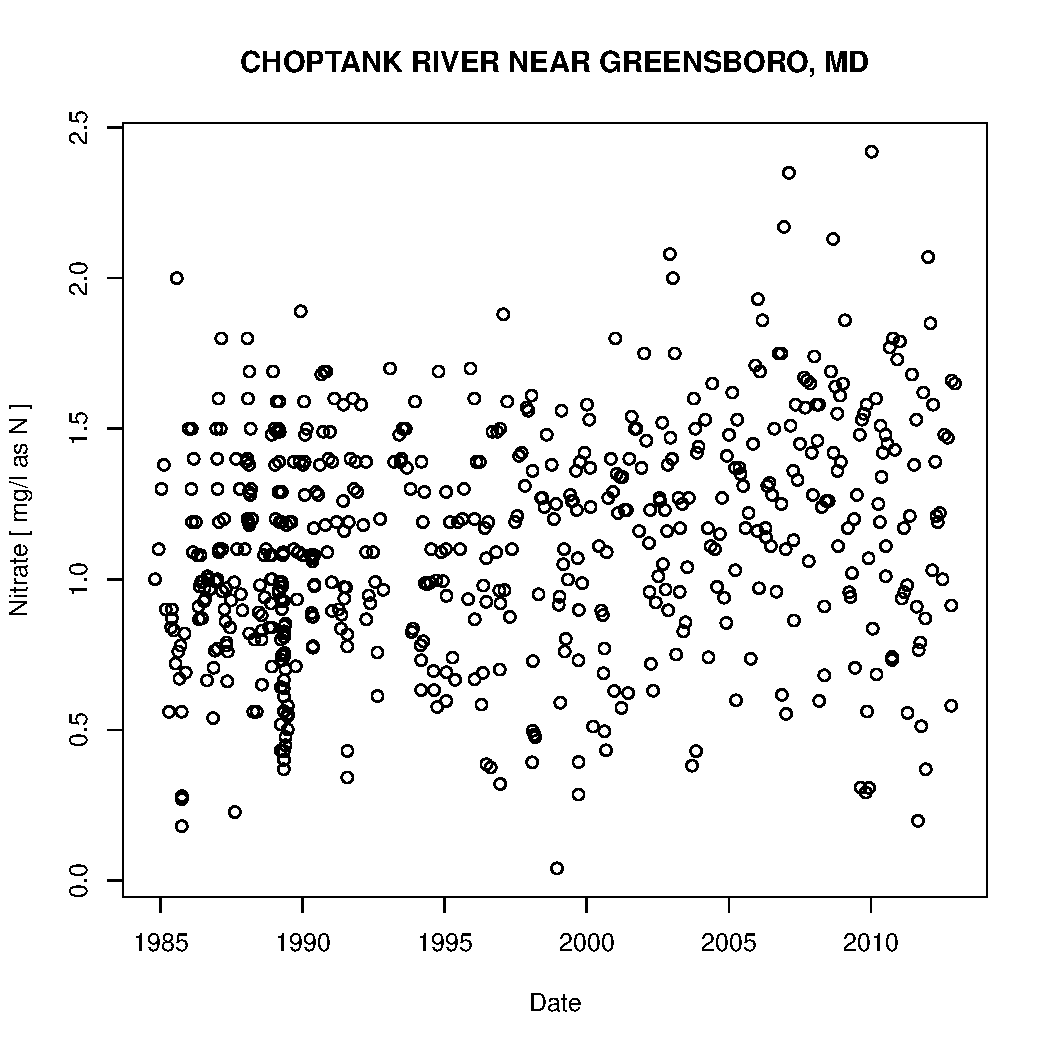
\includegraphics[width=\maxwidth]{figure/getQWtemperaturePlot} \caption[Nitrate plot of Choptank River]{Nitrate plot of Choptank River.\label{fig:getQWtemperaturePlot}}
\end{figure}


\end{knitrout}

\FloatBarrier

%------------------------------------------------------------
\subsection{STORET Water Quality Retrievals}
\label{sec:usgsSTORET}
%------------------------------------------------------------
There are additional water quality data sets available from the Water Quality Data Portal (\url{http://www.waterqualitydata.us/}).  These data sets can be housed in either the STORET (data from EPA) or NWIS database.  Since STORET does not use USGS parameter codes, a \texttt{"}characteristic name\texttt{"} must be supplied.  The \texttt{getWQPData} function can retrieve either STORET or NWIS, but requires a characteristic name rather than parameter code. The Water Quality Data Portal includes data discovery tools, and information on characteristic names. The following example retrieves specific conductance from a DNR site in Wisconsin. 


\begin{knitrout}
\definecolor{shadecolor}{rgb}{0.969, 0.969, 0.969}\color{fgcolor}\begin{kframe}
\begin{alltt}
\hlstd{specificCond} \hlkwb{<-} \hlkwd{getWQPData}\hlstd{(}\hlstr{'WIDNR_WQX-10032762'}\hlstd{,}
                \hlstr{'Specific conductance'}\hlstd{,}\hlstr{''}\hlstd{,}\hlstr{''}\hlstd{)}
\hlkwd{head}\hlstd{(specificCond)}
\end{alltt}
\begin{verbatim}
    dateTime qualifier. value.
1 2011-02-14              1360
2 2011-02-17              1930
3 2011-03-03              1240
4 2011-03-10              1480
5 2011-03-29              1130
6 2011-04-07              1200
\end{verbatim}
\end{kframe}
\end{knitrout}

There are 

\FloatBarrier
%------------------------------------------------------------
\subsection{URL Construction}
\label{sec:usgsURL}
%------------------------------------------------------------
There may be times when you might be interested in seeing the URL (Web address) that was used to obtain the raw data. The \texttt{constructNWISURL} function returns the URL.  In addition to input variables that have been described, there is a new argument \texttt{"}service\texttt{"}. The service argument can be \texttt{"}dv\texttt{"} (daily values), \texttt{"}uv\texttt{"} (unit values), \texttt{"}qw\texttt{"} (NWIS water quality values), or \texttt{"}wqp\texttt{"} (general Water Quality Portal values).
 

\begin{knitrout}
\definecolor{shadecolor}{rgb}{0.969, 0.969, 0.969}\color{fgcolor}\begin{kframe}
\begin{alltt}
\hlcom{# Dissolved Nitrate parameter codes:}
\hlstd{pCode} \hlkwb{<-} \hlkwd{c}\hlstd{(}\hlstr{"00618"}\hlstd{,}\hlstr{"71851"}\hlstd{)}
\hlstd{startDate} \hlkwb{<-} \hlstr{"1964-06-11"}
\hlstd{endDate} \hlkwb{<-} \hlstr{"2012-12-18"}
\hlstd{url_qw} \hlkwb{<-} \hlkwd{constructNWISURL}\hlstd{(siteNumber,pCode,startDate,endDate,}\hlstr{'qw'}\hlstd{)}
\hlstd{url_dv} \hlkwb{<-} \hlkwd{constructNWISURL}\hlstd{(siteNumber,}\hlstr{"00060"}\hlstd{,startDate,endDate,}
                           \hlstr{'dv'}\hlstd{,}\hlkwc{statCd}\hlstd{=}\hlstr{"00003"}\hlstd{)}
\hlstd{url_uv} \hlkwb{<-} \hlkwd{constructNWISURL}\hlstd{(siteNumber,}\hlstr{"00060"}\hlstd{,startDate,endDate,}\hlstr{'uv'}\hlstd{)}
\end{alltt}
\end{kframe}
\end{knitrout}

\FloatBarrier

%------------------------------------------------------------
\section{Data Retrievals Structured For Use In The EGRET Package}
\label{sec:EGRETdfs}
%------------------------------------------------------------ 
Rather than using the raw data as retrieved by the Web, the dataRetrieval package also includes functions that return the data in a structure that has been designed to work with the EGRET R package (\url{https://github.com/USGS-R/EGRET/wiki}). In general, these dataframes may be much more 'R-friendly' than the raw data, and will contain additional date information that allows for efficient data analysis.

In this section, we use 3 dataRetrieval functions to get sufficient data to perform an EGRET analysis.  We will continue analyzing the Choptank River. We will be retrieving essentially the same data that were retrieved in section \ref{sec:genRetrievals}, but in this case it will be structured into three EGRET-specific dataframes.  The daily discharge data will be placed in a dataframe called Daily.  The nitrate sample data will be placed in a dataframe called Sample.  The data about the site and the parameter will be placed in a dataframe called INFO.  Although these dataframes were designed to work with the EGRET R package, they can be very useful for a wide range of hydrology studies that don't use EGRET.

%------------------------------------------------------------
\subsection{INFO Data}
\label{INFOsubsection}
%------------------------------------------------------------
The \texttt{getMetaData} function obtains metadata, or data about the streamgage and measured parameters. This function combines \texttt{getSiteFileData} and \texttt{getParameterInfo}, producing one dataframe called INFO.

\begin{knitrout}
\definecolor{shadecolor}{rgb}{0.969, 0.969, 0.969}\color{fgcolor}\begin{kframe}
\begin{alltt}
\hlstd{parameterCd} \hlkwb{<-} \hlstr{"00618"}
\hlstd{INFO} \hlkwb{<-}\hlkwd{getMetaData}\hlstd{(siteNumber,parameterCd,} \hlkwc{interactive}\hlstd{=}\hlnum{FALSE}\hlstd{)}
\end{alltt}
\end{kframe}
\end{knitrout}


\FloatBarrier

%------------------------------------------------------------
\subsection{Daily Data}
\label{Dailysubsection}
%------------------------------------------------------------
The \texttt{getDVData} function retrieves the daily values (discharge in this case).  It requires the inputs siteNumber, parameterCd, startDate, endDate, interactive, and convert. Most of these arguments are described in section \ref{sec:genRetrievals}, however \texttt{"}convert\texttt{"} is a new argument (that defaults to TRUE). The convert argument tells the program to convert the values from cubic feet per second (ft\textsuperscript{3}/s) to cubic meters per second (m\textsuperscript{3}/s) as shown in the example Daily data frame in Table \ref{tab:DailyDF1}. For EGRET applications with NWIS Web retrieval, do not use this argument (the default is TRUE), EGRET assumes that discharge is always stored in units of cubic meters per second. If you don't want this conversion and are not using EGRET, set convert=FALSE in the function call. 

\begin{knitrout}
\definecolor{shadecolor}{rgb}{0.969, 0.969, 0.969}\color{fgcolor}\begin{kframe}
\begin{alltt}
\hlstd{siteNumber} \hlkwb{<-} \hlstr{"01491000"}
\hlstd{startDate} \hlkwb{<-} \hlstr{"2000-01-01"}
\hlstd{endDate} \hlkwb{<-} \hlstr{"2013-01-01"}
\hlcom{# This call will get NWIS (ft3/s) data , and convert it to m3/s:}
\hlstd{Daily} \hlkwb{<-} \hlkwd{getDVData}\hlstd{(siteNumber,} \hlstr{"00060"}\hlstd{, startDate, endDate)}
\end{alltt}
\begin{verbatim}
There are 4750 data points, and 4750 days.
\end{verbatim}
\end{kframe}
\end{knitrout}



% latex table generated in R 3.1.1 by xtable 1.7-3 package
% Tue Sep 09 09:13:21 2014
\begin{table}[ht]
\caption{Daily dataframe} 
\label{tab:DailyDF1}
{\footnotesize
\begin{tabular}{rllll}
  \hline
 & \multicolumn{1}{c}{\textbf{\textsf{ColumnName}}} & \multicolumn{1}{c}{\textbf{\textsf{Type}}} & \multicolumn{1}{c}{\textbf{\textsf{Description}}} & \multicolumn{1}{c}{\textbf{\textsf{Units}}} \\ 
  \hline
 & Date & Date & Date & date \\ 
  [5pt] & Q & number & Discharge in m3/s & m$^3$/s \\ 
  [5pt] & Julian & number & Number of days since January 1, 1850 & days \\ 
  [5pt] & Month & integer & Month of the year [1-12] & months \\ 
  [5pt] & Day & integer & Day of the year [1-366] & days \\ 
  [5pt] & DecYear & number & Decimal year & years \\ 
  [5pt] & MonthSeq & integer & Number of months since January 1, 1850 & months \\ 
  [5pt] & Qualifier & string & Qualifing code & character \\ 
  [5pt] & i & integer & Index of days, starting with 1 & days \\ 
  [5pt] & LogQ & number & Natural logarithm of Q & numeric \\ 
  [5pt] & Q7 & number & 7 day running average of Q & m$^3$/s \\ 
  [5pt] & Q30 & number & 30 day running average of Q & m$^3$/s \\ 
   \hline
\end{tabular}
}
\end{table}



If discharge values are negative or zero, the code will set all of these values to zero and then add a small constant to all of the daily discharge values.  This constant is 0.001 times the mean discharge.  The code will also report on the number of zero and negative values and the size of the constant.  Use EGRET analysis only if the number of zero values is a very small fraction of the total days in the record (say less than 0.1\% of the days), and there are no negative discharge values.  Columns Q7 and Q30 are the 7 and 30 day running averages for the 7 or 30 days ending on this specific date. Table \ref{tab:DailyDF1} lists details of the Daily data frame.

Notice that the \enquote{Day of the year} column can span from 1 to 366. The 366 accounts for leap years. Every day has a consistent day of the year. This means, February 28\textsuperscript{th} is always the 59\textsuperscript{th} day of the year, Feb. 29\textsuperscript{th} is always the 60\textsuperscript{th} day of the year, and March 1\textsuperscript{st} is always the 61\textsuperscript{st} day of the year whether or not it is a leap year.

\FloatBarrier

%------------------------------------------------------------
\subsection{Sample Data}
\label{Samplesubsection}
%------------------------------------------------------------
The \texttt{getSampleData} function retrieves USGS sample data from NWIS. The arguments for this function are also siteNumber, parameterCd, startDate, endDate, interactive. These are the same inputs as \texttt{retrieveWQPqwData} or \texttt{getWQPData} as described in the previous section.

\begin{knitrout}
\definecolor{shadecolor}{rgb}{0.969, 0.969, 0.969}\color{fgcolor}\begin{kframe}
\begin{alltt}
\hlstd{parameterCd} \hlkwb{<-} \hlstr{"00618"}
\hlstd{Sample} \hlkwb{<-}\hlkwd{getSampleData}\hlstd{(siteNumber,parameterCd,}
      \hlstd{startDate, endDate)}
\end{alltt}
\end{kframe}
\end{knitrout}

The \texttt{getSTORETSampleData} function retrieves STORET sample data (or other non-NWIS data) from the water quality portal. The arguments for this function are siteNumber, characteristicName, startDate, endDate, interactive. Table \ref{tab:SampleDataframe} lists details of the Sample data frame. 

\begin{knitrout}
\definecolor{shadecolor}{rgb}{0.969, 0.969, 0.969}\color{fgcolor}\begin{kframe}
\begin{alltt}
\hlstd{site} \hlkwb{<-} \hlstr{'WIDNR_WQX-10032762'}
\hlstd{characteristicName} \hlkwb{<-} \hlstr{'Specific conductance'}
\hlstd{Sample} \hlkwb{<-}\hlkwd{getSTORETSampleData}\hlstd{(site,characteristicName,}
      \hlstd{startDate, endDate)}
\end{alltt}
\end{kframe}
\end{knitrout}


\pagebreak


\begin{table}
{\footnotesize
  \begin{threeparttable}[b]
  \caption{Sample dataframe}
  \label{tab:SampleDataframe}
  \begin{tabular}{llll}
  \hline
\multicolumn{1}{c}{\textbf{\textsf{ColumnName}}} & 
\multicolumn{1}{c}{\textbf{\textsf{Type}}} & 
\multicolumn{1}{c}{\textbf{\textsf{Description}}} & 
\multicolumn{1}{c}{\textbf{\textsf{Units}}} \\ 
  \hline
  Date & Date & Date & date \\ 
  [5pt]ConcLow & number & Lower limit of concentration & mg/L \\ 
  [5pt]ConcHigh & number & Upper limit of concentration & mg/L \\ 
  [5pt]Uncen & integer & Uncensored data (1=true, 0=false) & integer \\ 
  [5pt]ConcAve & number & Average of ConcLow and ConcHigh & mg/L \\ 
  [5pt]Julian & number & Number of days since January 1, 1850 & days \\ 
  [5pt]Month & integer & Month of the year [1-12] & months \\ 
  [5pt]Day & integer & Day of the year [1-366] & days \\ 
  [5pt]DecYear & number & Decimal year & years \\ 
  [5pt]MonthSeq & integer & Number of months since January 1, 1850 & months \\ 
  [5pt]SinDY & number & Sine of DecYear & numeric \\ 
  [5pt]CosDY & number & Cosine of DecYear & numeric \\ 
  [5pt]Q \tnote{1} & number & Discharge & m\textsuperscript{3}/s \\ 
  [5pt]LogQ \tnote{1} & number & Natural logarithm of discharge & numeric \\ 
   \hline
\end{tabular}

  \begin{tablenotes}
    \item[1] Discharge columns are populated from data in the Daily dataframe after calling the \texttt{mergeReport} function.
  \end{tablenotes}
 \end{threeparttable}
}
\end{table}

Notice that the \enquote{Day of the year} column can span from 1 to 366. The 366 accounts for leap years. Every day has a consistent day of the year. This means, February 28\textsuperscript{th} is always the 59\textsuperscript{th} day of the year, Feb. 29\textsuperscript{th} is always the 60\textsuperscript{th} day of the year, and March 1\textsuperscript{st} is always the 61\textsuperscript{st} day of the year whether or not it is a leap year.

Section \ref{sec:cenValues} will talk about summing multiple constituents, including how interval censoring is used. Since the Sample data frame is structured to only contain one constituent, when more than one parameter codes are requested, the \texttt{getSampleData} function will sum the values of each constituent as described below.

\FloatBarrier


%------------------------------------------------------------
\subsection{Censored Values: Summation Explanation}
\label{sec:cenValues}
%------------------------------------------------------------
In the typical case where none of the data are censored (that is, no values are reported as \enquote{less-than} values) the ConcLow = ConcHigh = ConcAve and Uncen = 1 are equal to the reported value.  For the most common type of censoring, where a value is reported as less than the reporting limit, then ConcLow = NA, ConcHigh = reporting limit, ConcAve = 0.5 * reporting limit, and Uncen = 0.

To illustrate how the dataRetrieval package handles a more complex censoring problem, let us say that in 2004 and earlier, we computed total phosphorus (tp) as the sum of dissolved phosphorus (dp) and particulate phosphorus (pp). From 2005 and onward, we have direct measurements of total phosphorus (tp). A small subset of this fictional data looks like Table \ref{tab:exampleComplexQW}.



% latex table generated in R 3.1.1 by xtable 1.7-3 package
% Tue Sep 09 09:13:22 2014
\begin{table}[ht]
\caption{Example data} 
\label{tab:exampleComplexQW}
{\footnotesize
\begin{tabular}{rllrlrlr}
  \hline
 & \multicolumn{1}{c}{\textbf{\textsf{cdate}}} & \multicolumn{1}{c}{\textbf{\textsf{rdp}}} & \multicolumn{1}{c}{\textbf{\textsf{dp}}} & \multicolumn{1}{c}{\textbf{\textsf{rpp}}} & \multicolumn{1}{c}{\textbf{\textsf{pp}}} & \multicolumn{1}{c}{\textbf{\textsf{rtp}}} & \multicolumn{1}{c}{\textbf{\textsf{tp}}} \\ 
  \hline
 & 2003-02-15 &  & 0.020 &  & 0.500 &  &  \\ 
  [5pt] & 2003-06-30 & $<$ & 0.010 &  & 0.300 &  &  \\ 
  [5pt] & 2004-09-15 & $<$ & 0.005 & $<$ & 0.200 &  &  \\ 
  [5pt] & 2005-01-30 &  &  &  &  &  & 0.430 \\ 
  [5pt] & 2005-05-30 &  &  &  &  & $<$ & 0.050 \\ 
  [5pt] & 2005-10-30 &  &  &  &  & $<$ & 0.020 \\ 
   \hline
\end{tabular}
}
\end{table}


The dataRetrieval package will \enquote{add up} all the values in a given row to form the total for that sample when using the Sample dataframe. Thus, you only want to enter data that should be added together. If you want a dataframe with multiple constituents that are not summed, do not use getSampleData, getSTORETSampleData, or getSampleDataFromFile. The raw data functions: \texttt{getWQPData}, \texttt{retrieveNWISqwData}, \texttt{retrieveWQPqwData}, \texttt{getWQPData} will not sum constituents, but leave them in their individual columns. 

For example, we might know the value for dp on 5/30/2005, but we don't want to put it in the table because under the rules of this data set, we are not supposed to add it in to the values in 2005.

For every sample, the EGRET package requires a pair of numbers to define an interval in which the true value lies (ConcLow and ConcHigh). In a simple uncensored case (the reported value is above the detection limit), ConcLow equals ConcHigh and the interval collapses down to a single point. In a simple censored case, the value might be reported as \verb@<@0.2, then ConcLow=NA and ConcHigh=0.2. We use NA instead of 0 as a way to elegantly handle future logarithm calculations.

For the more complex example case, let us say dp is reported as \verb@<@0.01 and pp is reported as 0.3. We know that the total must be at least 0.3 and could be as much as 0.31. Therefore, ConcLow=0.3 and ConcHigh=0.31. Another case would be if dp is reported as \verb@<@0.005 and pp is reported \verb@<@0.2. We know in this case that the true value could be as low as zero, but could be as high as 0.205. Therefore, in this case, ConcLow=NA and ConcHigh=0.205. The Sample dataframe for the example data would be:



\begin{knitrout}
\definecolor{shadecolor}{rgb}{0.969, 0.969, 0.969}\color{fgcolor}\begin{kframe}
\begin{alltt}
  \hlstd{Sample}
\end{alltt}
\begin{verbatim}
        Date ConcLow ConcHigh Uncen ConcAve Julian Month
1 2003-02-15    0.52    0.520     1  0.5200  55927     2
2 2003-06-30    0.30    0.310     0  0.3050  56062     6
3 2004-09-15      NA    0.205     0  0.1025  56505     9
4 2005-01-30    0.43    0.430     1  0.4300  56642     1
5 2005-05-30      NA    0.050     0  0.0250  56762     5
6 2005-10-30      NA    0.020     0  0.0100  56915    10
  Day DecYear MonthSeq    SinDY   CosDY
1  46    2003     1838  0.70253  0.7117
2 182    2003     1842  0.03872 -0.9993
3 259    2005     1857 -0.96134 -0.2754
4  30    2005     1861  0.48251  0.8759
5 151    2005     1865  0.54163 -0.8406
6 304    2006     1870 -0.88205  0.4712
\end{verbatim}
\end{kframe}
\end{knitrout}

Section \ref{sec:userFiles} discusses inputting user-generated files. The functions \texttt{getSampleDataFromFile} and \texttt{getSampleData} assume summation with interval censoring inputs, and are discussed in sections \ref{sec:DailyFile} and \ref{sec:SampleFile}.

\FloatBarrier

%------------------------------------------------------------ 
\subsection{User-Generated Data Files}
\label{sec:userFiles}
%------------------------------------------------------------ 
In addition to retrieving data from the USGS Web services, the dataRetrieval package also includes functions to generate the Daily and Sample data frame from local files.

%------------------------------------------------------------ 
\subsubsection{getDailyDataFromFile}
\label{sec:DailyFile}
%------------------------------------------------------------ 
The \texttt{getDailyDataFromFile} function will load a user-supplied text file and convert it to the Daily dataframe. The file should have two columns, the first dates, the second values.  The dates are formatted either mm/dd/yyyy or yyyy-mm-dd. Using a 4-digit year is required. This function has the following inputs: filePath, fileName,hasHeader (TRUE/FALSE), separator, qUnit, and interactive (TRUE/FALSE). filePath is a string that defines the path to your file, and the string can either be a full path, or path relative to your R working directory. The input fileName is a string that defines the file name (including the extension).

Text files that contain this sort of data require some sort of a separator, for example, a \enquote{csv} file (comma-separated value) file uses a comma to separate the date and value column. A tab delimited file would use a tab (\verb@"\t"@) rather than the comma (\texttt{"},\texttt{"}). Define the type of separator you choose to use in the function call in the \texttt{"}separator\texttt{"} argument, the default is \texttt{"},\texttt{"}. Another function input is a logical variable: hasHeader.  The default is TRUE. If your data does not have column names, set this variable to FALSE.

Finally, qUnit is a numeric argument that defines the discharge units used in the input file.  The default is qUnit = 1 which assumes discharge is in cubic feet per second.  If the discharge in the file is already in cubic meters per second then set qUnit = 2.  If it is in some other units (like liters per second or acre-feet per day), the user must pre-process the data with a unit conversion that changes it to either cubic feet per second or cubic meters per second.

So, if you have a file called \enquote{ChoptankRiverFlow.txt} located in a folder called \enquote{RData} on the C drive (this is a Windows example), and the file is structured as follows (tab-separated):


\singlespacing
\begin{verbatim}
date  Qdaily
10/1/1999  107
10/2/1999  85
10/3/1999	76
10/4/1999	76
10/5/1999	113
10/6/1999	98
...
\end{verbatim}
\doublespacing

The call to open this file, convert the discharge to cubic meters per second, and populate the Daily data frame would be:
\begin{knitrout}
\definecolor{shadecolor}{rgb}{0.969, 0.969, 0.969}\color{fgcolor}\begin{kframe}
\begin{alltt}
\hlstd{fileName} \hlkwb{<-} \hlstr{"ChoptankRiverFlow.txt"}
\hlstd{filePath} \hlkwb{<-}  \hlstr{"C:/RData/"}
\hlstd{Daily} \hlkwb{<-} \hlkwd{getDailyDataFromFile}\hlstd{(filePath,fileName,}
                    \hlkwc{separator}\hlstd{=}\hlstr{"\textbackslash{}t"}\hlstd{)}
\end{alltt}
\end{kframe}
\end{knitrout}

Microsoft Excel files can be a bit tricky to import into R directly. The simplest way to get Excel data into R is to open the Excel file in Excel, then save it as a .csv file (comma-separated values). 

\FloatBarrier

%------------------------------------------------------------ 
\subsubsection{getSampleDataFromFile}
\label{sec:SampleFile}
%------------------------------------------------------------ 

\doublespacing
The \texttt{getSampleDataFromFile} function will import a user-generated file and populate the Sample dataframe. The difference between sample data and discharge data is that the code requires a third column that contains a remark code, either blank or \verb@"<"@, which will tell the program that the data was \enquote{left-censored} (or, below the detection limit of the sensor). Therefore, the data must be in the form: date, remark, value.   An example of a comma-delimited file is:

\singlespacing
\begin{verbatim}
cdate;remarkCode;Nitrate
10/7/1999,,1.4
11/4/1999,<,0.99
12/3/1999,,1.42
1/4/2000,,1.59
2/3/2000,,1.54
...
\end{verbatim}
\doublespacing

The call to open this file, and populate the Sample dataframe is:
\begin{knitrout}
\definecolor{shadecolor}{rgb}{0.969, 0.969, 0.969}\color{fgcolor}\begin{kframe}
\begin{alltt}
\hlstd{fileName} \hlkwb{<-} \hlstr{"ChoptankRiverNitrate.csv"}
\hlstd{filePath} \hlkwb{<-}  \hlstr{"C:/RData/"}
\hlstd{Sample} \hlkwb{<-} \hlkwd{getSampleDataFromFile}\hlstd{(filePath,fileName,}
                                \hlkwc{separator}\hlstd{=}\hlstr{","}\hlstd{)}
\end{alltt}
\end{kframe}
\end{knitrout}

When multiple constituents are to be summed, the format can be date, remark\_A, value\_A, remark\_b, value\_b, etc... A tab-separated example might look like the file below, where the columns are date, remark dissolved phosphate (rdp), dissolved phosphate (dp), remark particulate phosphorus (rpp), particulate phosphorus (pp), remark total phosphate (rtp), and total phosphate (tp):

\singlespacing
\begin{verbatim}
date  rdp	dp	rpp	pp	rtp	tp
2003-02-15		0.020		0.500		
2003-06-30	<	0.010		0.300		
2004-09-15	<	0.005	<	0.200		
2005-01-30						0.430
2005-05-30					<	0.050
2005-10-30					<	0.020
...
\end{verbatim}
\doublespacing
\begin{knitrout}
\definecolor{shadecolor}{rgb}{0.969, 0.969, 0.969}\color{fgcolor}\begin{kframe}
\begin{alltt}
\hlstd{fileName} \hlkwb{<-} \hlstr{"ChoptankPhosphorus.txt"}
\hlstd{filePath} \hlkwb{<-}  \hlstr{"C:/RData/"}
\hlstd{Sample} \hlkwb{<-} \hlkwd{getSampleDataFromFile}\hlstd{(filePath,fileName,}
                                \hlkwc{separator}\hlstd{=}\hlstr{"\textbackslash{}t"}\hlstd{)}
\end{alltt}
\end{kframe}
\end{knitrout}


\FloatBarrier

%------------------------------------------------------------
\subsection{Merge Report}
%------------------------------------------------------------
Finally, there is a function called \texttt{mergeReport} that will look at both the Daily and Sample dataframe, and populate Q and LogQ columns into the Sample dataframe. The default arguments are Daily and Sample, however if you want to use other similarly structured dataframes, you can specify localDaily or localSample. Once \texttt{mergeReport} has been run, the Sample dataframe will be augmented with the daily discharges for all the days with samples.  None of the water quality functions in EGRET will work without first having run the \texttt{mergeReport} function.


\begin{knitrout}
\definecolor{shadecolor}{rgb}{0.969, 0.969, 0.969}\color{fgcolor}\begin{kframe}
\begin{alltt}
\hlstd{siteNumber} \hlkwb{<-} \hlstr{"01491000"}
\hlstd{parameterCd} \hlkwb{<-} \hlstr{"00631"}  \hlcom{# Nitrate}
\hlstd{startDate} \hlkwb{<-} \hlstr{"2000-01-01"}
\hlstd{endDate} \hlkwb{<-} \hlstr{"2013-01-01"}

\hlstd{Daily} \hlkwb{<-} \hlkwd{getDVData}\hlstd{(siteNumber,} \hlstr{"00060"}\hlstd{, startDate, endDate)}
\end{alltt}
\begin{verbatim}
There are 4750 data points, and 4750 days.
\end{verbatim}
\begin{alltt}
\hlstd{Sample} \hlkwb{<-} \hlkwd{getSampleData}\hlstd{(siteNumber,parameterCd, startDate, endDate)}
\hlstd{Sample} \hlkwb{<-} \hlkwd{mergeReport}\hlstd{()}
\end{alltt}
\begin{verbatim}

 Discharge Record is 4750 days long, which is 13 years
 First day of the discharge record is 2000-01-01 and last day is 2013-01-01
 The water quality record has 222 samples
 The first sample is from 2000-01-04 and the last sample is from 2012-12-18
 Discharge: Minimum, mean and maximum 0.00991 4.55 246
 Concentration: Minimum, mean and maximum 0.2 1.2 2.4
 Percentage of the sample values that are censored is 0 %
\end{verbatim}
\begin{alltt}
\hlkwd{head}\hlstd{(Sample)}
\end{alltt}
\begin{verbatim}
        Date      Q   LogQ ConcLow ConcHigh Uncen ConcAve
1 2000-01-04  2.747 1.0104    1.59     1.59     1    1.59
2 2000-02-03  3.936 1.3702    1.54     1.54     1    1.54
3 2000-02-15 10.845 2.3837    1.37     1.37     1    1.37
4 2000-02-19 15.518 2.7420    1.24     1.24     1    1.24
5 2000-03-23 56.917 4.0416    0.52     0.52     1    0.52
6 2000-06-05  1.812 0.5946    1.11     1.11     1    1.11
  Julian Month Day DecYear MonthSeq   SinDY   CosDY
1  54789     1   4    2000     1801 0.05576  0.9984
2  54819     2  34    2000     1802 0.54031  0.8415
3  54831     2  46    2000     1802 0.70101  0.7132
4  54835     2  50    2000     1802 0.74829  0.6634
5  54868     3  83    2000     1803 0.98742  0.1581
6  54942     6 157    2000     1806 0.44325 -0.8964
\end{verbatim}
\end{kframe}
\end{knitrout}

\FloatBarrier

%------------------------------------------------------------
\subsection{EGRET Plots}
%------------------------------------------------------------
The Daily, Sample, and INFO data frames (described in Secs. \ref{INFOsubsection} - \ref{Samplesubsection}) are specifically formatted to be used with the EGRET package. The EGRET package has powerful modeling capabilities that use WRTDS, but EGRET also has graphing and tabular tools for exploring the data without using the WRTDS algorithm. See the EGRET vignette, user guide, and/or wiki (\url{https://github.com/USGS-R/EGRET/wiki}) for detailed information. Figure \ref{fig:egretEx} shows one of the plotting functions that can be used directly from the dataRetrieval dataframes.

\begin{knitrout}
\definecolor{shadecolor}{rgb}{0.969, 0.969, 0.969}\color{fgcolor}\begin{kframe}
\begin{alltt}
\hlcom{# Continuing Choptank example from the previous sections}
\hlkwd{library}\hlstd{(EGRET)}
\hlkwd{multiPlotDataOverview}\hlstd{()}
\end{alltt}
\end{kframe}\begin{figure}[]

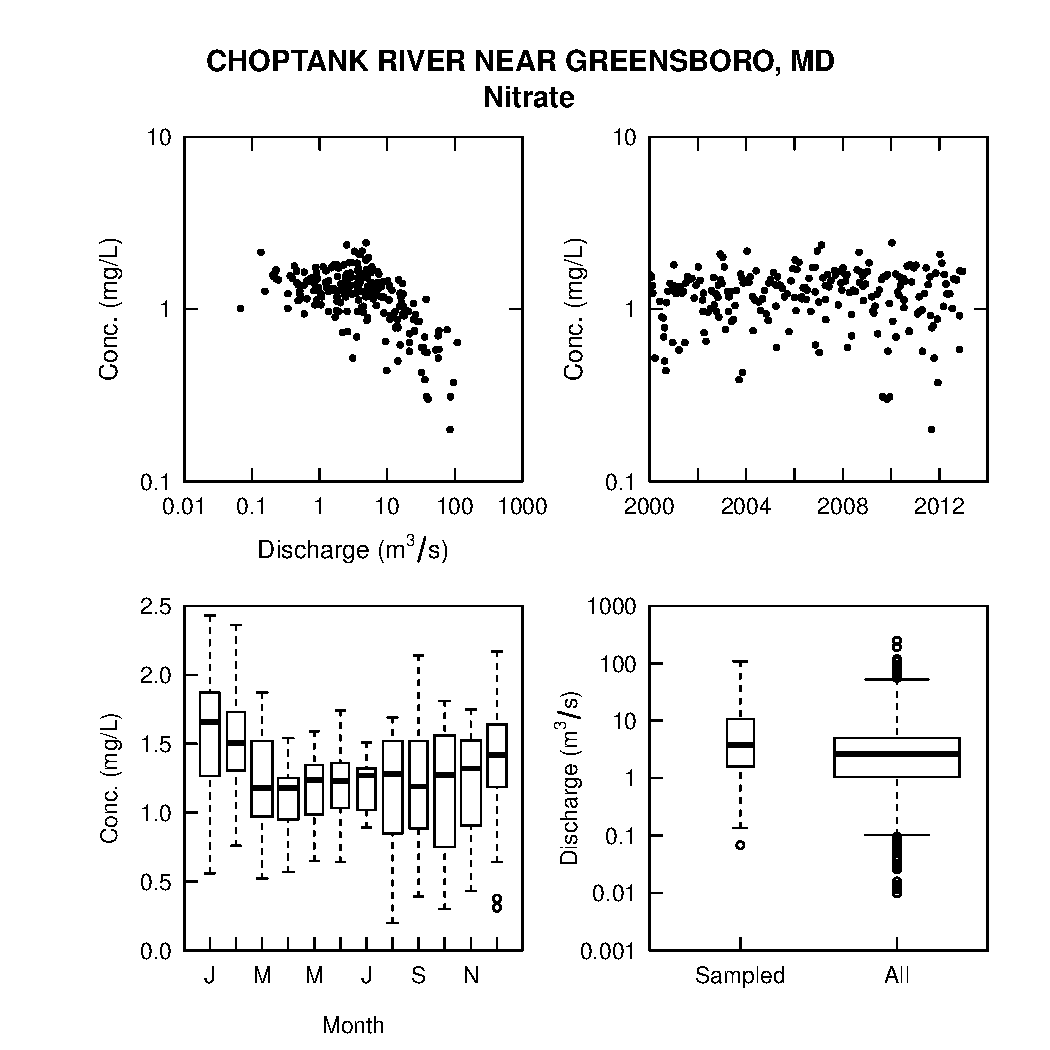
\includegraphics[width=\maxwidth]{figure/egretEx} \caption[Default multiPlotDataOverview]{Default multiPlotDataOverview\label{fig:egretEx}}
\end{figure}


\end{knitrout}

\FloatBarrier
\clearpage


%------------------------------------------------------------
\section{Summary}
\label{sec:summary}
%------------------------------------------------------------

Tables \ref{tab:dataRetrievalFunctions1} and \ref{tab:dataRetrievalMisc} summarize the data retrieval functions:

\begin{table}
{\footnotesize
  \begin{threeparttable}[b]
  \caption{dataRetrieval functions}
  \label{tab:dataRetrievalFunctions1}
%   \doublespacing
\begin{tabular}{lll}
  \hline
\multicolumn{1}{c}{\textbf{\textsf{Data Type}}} &
\multicolumn{1}{c}{\textbf{\textsf{Function Name}}} &
\multicolumn{1}{c}{\textbf{\textsf{Description}}} \\ [0pt]
  \hline
  Daily & \texttt{retrieveNWISdvData} & Raw USGS daily data \\ 
  [5pt]Daily\tnote{1} & \texttt{getDVData} & USGS daily values \\ 
  [5pt]Daily\tnote{1} & \texttt{getDailyDataFromFile} & User generated daily data \\ 
  [5pt]Sample & \texttt{retrieveNWISqwData} & Raw USGS water quality data \\
  [5pt]Sample & \texttt{retrieveWQPqwData} & Raw Water Quality Data Portal data \\ 
  [5pt]Sample & \texttt{getQWDataFromFile} & Raw user generated water quality data \\ 
  [5pt]Sample & \texttt{getWQPData} & General Water Quality Portal\\
  [5pt]Sample\tnote{1} & \texttt{getSampleData} & USGS water quality data\\
  [5pt]Sample\tnote{1} & \texttt{getSTORETSampleData} & STORET Water Quality Data Portal data \\
  [5pt]Sample\tnote{1} & \texttt{getSampleDataFromFile} & User generated sample data \\ 
  [5pt]Unit & \texttt{retrieveNWISunitData} & Raw USGS instantaneous data \\
  [5pt]Information\tnote{1} & \texttt{getMetaData} & USGS station and parameter code information \\ 
  [5pt]Information & \texttt{getParameterInfo} & USGS parameter code information \\ 
  [5pt]Information & \texttt{getSiteFileData} & USGS station information \\ 
  [5pt]Information & \texttt{getDataAvailability} & Data available at USGS stations \\ 
   \hline
\end{tabular}

  \begin{tablenotes}
    \item[1] Indicates that the function creates a data frame suitable for use in EGRET software
  \end{tablenotes}
 \end{threeparttable}
}
\end{table}


\begin{table}[!ht]
\begin{minipage}{\linewidth}
{\footnotesize
\caption{dataRetrieval miscellaneous functions} 
\label{tab:dataRetrievalMisc}
\begin{tabular}{ll}
  \hline
\multicolumn{1}{c}{\textbf{\textsf{Function Name}}} &
\multicolumn{1}{c}{\textbf{\textsf{Description}}} \\  [0pt]
  \hline
  \texttt{compressData} &  Converts value/qualifier into ConcLow, ConcHigh, Uncen\\
  [5pt]\texttt{getRDB1Data} & Retrieves and converts RDB data to dataframe\\
  [5pt]\texttt{getWaterML1Data} & Retrieves and converts WaterML1 data to dataframe\\
  [5pt]\texttt{getWaterML2Data} & Retrieves and converts WaterML2 data to dataframe\\
  [5pt]\texttt{mergeReport} & Merges flow data from the daily record into the sample record\\
  [5pt]\texttt{populateDateColumns} & Generates Julian, Month, Day, DecYear, and MonthSeq columns\\
  [5pt]\texttt{removeDuplicates} & Removes duplicated rows\\
  [5pt]\texttt{renameColumns} & Renames columns from raw data retrievals\\
   \hline
\end{tabular}
}
\end{minipage}
\end{table}

\FloatBarrier
\clearpage


%------------------------------------------------------------ 
\section{Getting Started in R}
\label{sec:appendix1}
%------------------------------------------------------------ 
This section describes the options for downloading and installing the dataRetrieval package.

%------------------------------------------------------------
\subsection{New to R?}
%------------------------------------------------------------ 
If you are new to R, you will need to first install the latest version of R, which can be found here: \url{http://www.r-project.org/}.

At any time, you can get information about any function in R by typing a question mark before the functions name.  This will open a file (in RStudio, in the Help window) that describes the function, the required arguments, and provides working examples.

\begin{knitrout}
\definecolor{shadecolor}{rgb}{0.969, 0.969, 0.969}\color{fgcolor}\begin{kframe}
\begin{alltt}
\hlopt{?}\hlstd{removeDuplicates}
\end{alltt}
\end{kframe}
\end{knitrout}

This will open a help file similar to Figure \ref{fig:help}.

\FloatBarrier

To see the raw code for a particular code, type the name of the function, without parentheses.:
\begin{knitrout}
\definecolor{shadecolor}{rgb}{0.969, 0.969, 0.969}\color{fgcolor}\begin{kframe}
\begin{alltt}
\hlstd{removeDuplicates}
\end{alltt}
\begin{verbatim}
function (localSample = Sample) 
{
    Sample1 <- localSample[!duplicated(localSample[c("DecYear", 
        "ConcHigh")]), ]
    return(Sample1)
}
<environment: namespace:dataRetrieval>
\end{verbatim}
\end{kframe}
\end{knitrout}


\begin{figure}[ht!]
\centering
 \resizebox{0.95\textwidth}{!}{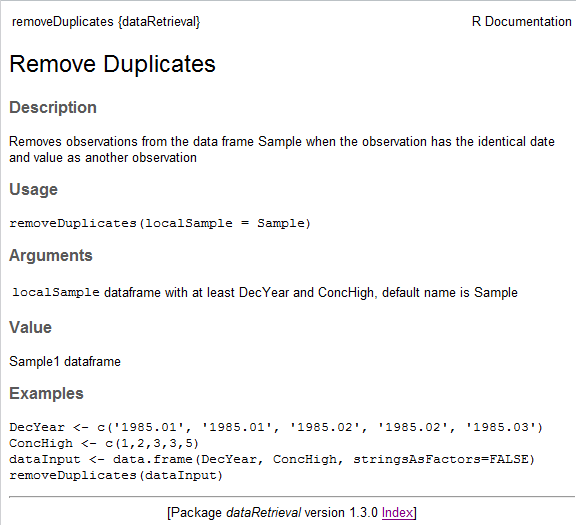
\includegraphics{Rhelp.png}} 
\caption{A simple R help file}
\label{fig:help}
\end{figure}

Additionally, many R packages have vignette files attached (such as this paper). To view the vignette:
\begin{knitrout}
\definecolor{shadecolor}{rgb}{0.969, 0.969, 0.969}\color{fgcolor}\begin{kframe}
\begin{alltt}
\hlkwd{vignette}\hlstd{(dataRetrieval)}
\end{alltt}
\end{kframe}
\end{knitrout}

\FloatBarrier
\clearpage
%------------------------------------------------------------
\subsection{R User: Installing dataRetrieval}
%------------------------------------------------------------ 
The following command installs dataRetrieval and subsequent required packages:

\begin{knitrout}
\definecolor{shadecolor}{rgb}{0.969, 0.969, 0.969}\color{fgcolor}\begin{kframe}
\begin{alltt}
\hlkwd{install.packages}\hlstd{(}\hlstr{"dataRetrieval"}\hlstd{,}
\hlkwc{repos}\hlstd{=}\hlkwd{c}\hlstd{(}\hlstr{"http://usgs-r.github.com"}\hlstd{,}\hlstr{"http://cran.us.r-project.org"}\hlstd{),}
\hlkwc{dependencies}\hlstd{=}\hlnum{TRUE}\hlstd{,}
\hlkwc{type}\hlstd{=}\hlstr{"both"}\hlstd{)}
\end{alltt}
\end{kframe}
\end{knitrout}

After installing the package, you need to open the library each time you re-start R.  This is done with the simple command:
\begin{knitrout}
\definecolor{shadecolor}{rgb}{0.969, 0.969, 0.969}\color{fgcolor}\begin{kframe}
\begin{alltt}
\hlkwd{library}\hlstd{(dataRetrieval)}
\end{alltt}
\end{kframe}
\end{knitrout}


%------------------------------------------------------------ 
\section{Creating tables in Microsoft from R}
\label{app:createWordTable}
%------------------------------------------------------------
There are a few steps that are required in order to create a table in a Microsoft product (Excel, Word, Powerpoint, etc.) from an R dataframe. There are certainly a variety of good methods, one of which is detailed here. The example we will step through here will be to create a table in Microsoft Excel based on the dataframe tableData:

\begin{knitrout}
\definecolor{shadecolor}{rgb}{0.969, 0.969, 0.969}\color{fgcolor}\begin{kframe}
\begin{alltt}
\hlstd{availableData} \hlkwb{<-} \hlkwd{getDataAvailability}\hlstd{(siteNumber)}
\hlstd{dailyData} \hlkwb{<-} \hlstd{availableData[}\hlstr{"dv"} \hlopt{==} \hlstd{availableData}\hlopt{$}\hlstd{service,]}
\hlstd{dailyData} \hlkwb{<-} \hlstd{dailyData[}\hlstr{"00003"} \hlopt{==} \hlstd{dailyData}\hlopt{$}\hlstd{statCd,]}

\hlstd{tableData} \hlkwb{<-} \hlkwd{with}\hlstd{(dailyData,}
      \hlkwd{data.frame}\hlstd{(}
        \hlkwc{shortName}\hlstd{=srsname,}
        \hlkwc{Start}\hlstd{=startDate,}
        \hlkwc{End}\hlstd{=endDate,}
        \hlkwc{Count}\hlstd{=count,}
        \hlkwc{Units}\hlstd{=parameter_units)}
      \hlstd{)}
\hlstd{tableData}
\end{alltt}
\begin{verbatim}
                               shortName      Start
1                     Temperature, water 2010-10-01
2               Stream flow, mean. daily 1948-01-01
3                   Specific conductance 2010-10-01
4 Suspended sediment concentration (SSC) 1980-10-01
5           Suspended sediment discharge 1980-10-01
         End Count      Units
1 2012-05-09   529      deg C
2 2014-09-07 24357      ft3/s
3 2012-05-09   527 uS/cm @25C
4 1991-09-30  3651       mg/l
5 1991-09-30  3652   tons/day
\end{verbatim}
\end{kframe}
\end{knitrout}

First, save the dataframe as a tab delimited file (you don't want to use comma delimited because there are commas in some of the data elements):


\begin{knitrout}
\definecolor{shadecolor}{rgb}{0.969, 0.969, 0.969}\color{fgcolor}\begin{kframe}
\begin{alltt}
\hlkwd{write.table}\hlstd{(tableData,} \hlkwc{file}\hlstd{=}\hlstr{"tableData.tsv"}\hlstd{,}\hlkwc{sep}\hlstd{=}\hlstr{"\textbackslash{}t"}\hlstd{,}
            \hlkwc{row.names} \hlstd{=} \hlnum{FALSE}\hlstd{,}\hlkwc{quote}\hlstd{=}\hlnum{FALSE}\hlstd{)}
\end{alltt}
\end{kframe}
\end{knitrout}

This will save a file in your working directory called tableData.tsv.  You can see your working directory by typing getwd() in the R console. Opening the file in a general-purpose text editor, you should see the following:

\begin{verbatim}
shortName  Start  End	Count	Units
Temperature, water	2010-10-01	2012-06-24	575	deg C
Stream flow, mean. daily	1948-01-01	2013-03-13	23814	ft3/s
Specific conductance	2010-10-01	2012-06-24	551	uS/cm @25C
Suspended sediment concentration (SSC)	1980-10-01	1991-09-30	3651	mg/l
Suspended sediment discharge	1980-10-01	1991-09-30	3652	tons/day
\end{verbatim}

Next, follow the steps below to open this file in Excel:
\begin{enumerate}
\item Open Excel
\item Click on the File tab
\item Click on the Open option
\item Navigate to the working directory (as shown in the results of getwd())
\item Next to the File name text box, change the dropdown type to All Files (*.*)
\item Double click tableData.tsv
\item A text import wizard will open up, in the first window, choose the Delimited radio button if it is not automatically picked, then click on Next.
\item In the second window, click on the Tab delimiter if it is not automatically checked, then click Finished.
\item Use the many formatting tools within Excel to customize the table
\end{enumerate}

From Excel, it is simple to copy and paste the tables in other Microsoft products. An example using one of the default Excel table formats is here.

\begin{figure}[ht!]
\centering
 \resizebox{0.9\textwidth}{!}{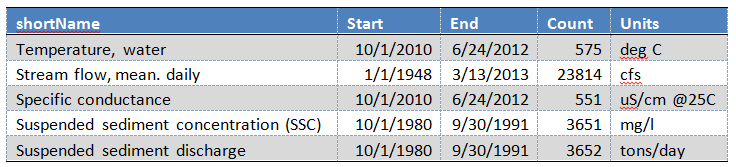
\includegraphics{table1.png}} 
\caption{A simple table produced in Microsoft Excel}
\label{overflow}
\end{figure}

\clearpage

% %------------------------------------------------------------
% % BIBLIO
% %------------------------------------------------------------
% \begin{thebibliography}{10}
% 
% \bibitem{HirschI}
% Helsel, D.R. and R. M. Hirsch, 2002. Statistical Methods in Water Resources Techniques of Water Resources Investigations, Book 4, chapter A3. U.S. Geological Survey. 522 pages. \url{http://pubs.usgs.gov/twri/twri4a3/}
% 
% \bibitem{HirschII}
% Hirsch, R. M., Moyer, D. L. and Archfield, S. A. (2010), Weighted Regressions on Time, Discharge, and Season (WRTDS), with an Application to Chesapeake Bay River Inputs. JAWRA Journal of the American Water Resources Association, 46: 857-880. doi: 10.1111/j.1752-1688.2010.00482.x \url{http://onlinelibrary.wiley.com/doi/10.1111/j.1752-1688.2010.00482.x/full}
% 
% \bibitem{HirschIII}
% Sprague, L. A., Hirsch, R. M., and Aulenbach, B. T. (2011), Nitrate in the Mississippi River and Its Tributaries, 1980 to 2008: Are We Making Progress? Environmental Science \& Technology, 45 (17): 7209-7216. doi: 10.1021/es201221s \url{http://pubs.acs.org/doi/abs/10.1021/es201221s}
% 
% \end{thebibliography}

% \end{document}

\end{document}
